\documentclass[10pt,a4paper]{article}

\usepackage[T1]{fontenc}
\usepackage[utf8]{inputenc}
\usepackage{charter}
\usepackage[margin=19mm,top=17mm,bottom=18mm]{geometry}
\usepackage{booktabs}
\usepackage{enumitem}
\usepackage{microtype}
\usepackage{titlesec}
\usepackage{amsmath}
\usepackage{fancyhdr}
\usepackage{tikz}
\usetikzlibrary{arrows.meta,positioning,fit,backgrounds}
\usepackage[hidelinks]{hyperref}

\titleformat{\section}{\bfseries\large}{\thesection.}{0.5em}{}
\titleformat{\subsection}{\bfseries\normalsize}{\thesubsection}{0.5em}{}
\titlespacing*{\section}{0pt}{9pt plus 2pt minus 2pt}{4pt}
\titlespacing*{\subsection}{0pt}{7pt plus 2pt minus 2pt}{3pt}

\setlist[itemize]{leftmargin=13pt,itemsep=1pt,topsep=3pt,parsep=0pt}
\setlist[enumerate]{leftmargin=16pt,itemsep=1pt,topsep=3pt,parsep=0pt}

\pagestyle{fancy}
\fancyhf{}
\renewcommand{\headrulewidth}{0.4pt}
\lhead{\small Escalate, Don't Replace --- HSBC Challenge Statement}
\rhead{\small \thepage}

\setlength{\parskip}{3.5pt}
\setlength{\parindent}{0pt}

\begin{document}

\begin{center}
{\large\bfseries Escalate, Don't Replace}\\[2pt]
{\large\bfseries A Budget-Routed Quantum--Classical Detector for Card-Not-Present Fraud,}\\
{\large\bfseries with Falsification Built Into the Protocol}\\[6pt]
{\small Global Quantum + AI Challenge 2026 --- Phase 1 Concept Proposal\\
Enterprise Problem Statement: HSBC, \emph{Quantum-Enhanced Credit Card Fraud Detection for Digital Payment Ecosystems}\\[3pt]
Akshit Agarwal (Lead Researcher) --- Rashtriya Raksha University, Gandhinagar, India}
\end{center}

\vspace{2pt}
\hrule
\vspace{6pt}

\section{Problem Framing}

The published quantum results on this exact problem look better than they are, and the reason is the evaluation protocol rather than the physics.

Kyriienko and Magnusson report quantum kernels beating RBF kernels by more than ten percentage points of average precision --- on 500 transactions containing 25 frauds, deliberately rebalanced~[7]. Innan et al.\ report a QSVC F1 of 0.98~[6]. Bhutta and Mehmood report simulated quantum F1 scores approaching 1.000, on a 50/50 balanced variant of a dataset whose true fraud rate is 0.172\%~[9]. CircuitHunt reaches 97\% test accuracy after SMOTE balancing~[5]. None of these numbers survives contact with a 0.172\% base rate and a temporally ordered test set, and none of the papers claims otherwise --- the claims are being made by readers, not authors.

The one study that measured carefully found something much more modest. Chaves et al.\ route transactions selectively to a hybrid quantum expert and report average precision of $0.793 \pm 0.085$ against $0.770 \pm 0.096$ for XGBoost over three repeated 5-fold benchmarks~[1]. The intervals overlap almost entirely. The honest summary of the field in September 2026 is: \emph{no demonstrated advantage on realistic fraud data, but a converging architecture.}

That architecture is worth taking seriously, because industry reached it independently. OQC and Mastercard route only the hardest and highest-value transactions to quantum hardware and leave classical models on everything else, precisely to stay inside the latency envelope; they report reduced false positives from the arrangement~[2]. Chaves et al.\ describe the same shape. Nobody is proposing to replace the gradient-boosted ensemble. Everyone is proposing to escalate a sliver of traffic to it.

We think the escalation fraction is the interesting variable, and nobody is treating it as one.

Fix a budget $B$ --- the share of transactions allowed to reach the quantum expert --- and the awkward properties of near-term quantum models stop being disqualifying. A model that needs 200\,ms cannot sit inside a 100--300\,ms authorization path for every transaction; Mastercard's network response alone averages 130\,ms. It can sit there for 1\% of transactions if the other 99\% clear in microseconds. Shot cost, qubit count and circuit depth all scale with $B$, not with volume. Meanwhile the property quantum kernels are actually conjectured to have --- better generalization from very few labelled examples --- applies exactly where the classical model is already weakest: the uncertain band near the decision boundary, where fraud examples are sparse and the boosted trees are guessing.

There is a second thing the literature under-weights. HSBC's own figures make fraud economically asymmetric: \$4.41 of cost per \$1 of fraud once investigation is included, \$443bn of legitimate transactions falsely declined, and more than 40\% of customers abandoning a purchase after a decline. AUPRC treats a false positive and a false negative as commensurable. A bank does not. We will report a cost-weighted metric alongside the standard ones.

So the question we propose to answer is narrow and answerable in a PoC sprint: \textbf{at what escalation budget, if any, does a quantum expert change the precision--recall trade-off on temporally split card-not-present data by more than a tuned classical expert in the same slot would?} We have designed the experiment so that ``never'' is a publishable answer.

\section{Technical Approach}

\textbf{Paradigm.} Hybrid classical--quantum, gate-based. Two quantum experts are evaluated: one non-variational (projected quantum kernel), one variational (quantum autoencoder scored by state fidelity). A quantum-inspired tensor-network arm serves as a diagnostic, not as a competitor.

\begin{figure}[h]
\centering
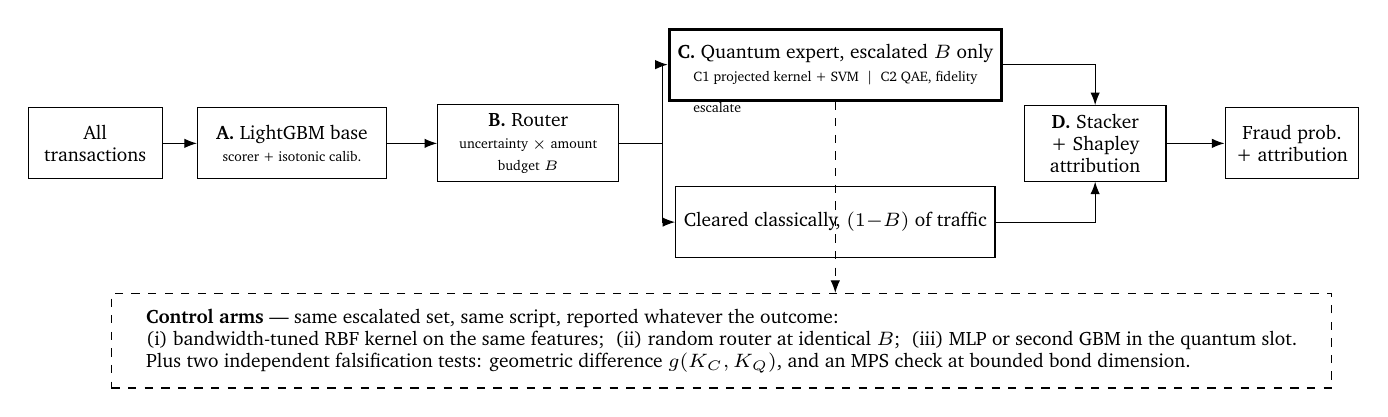
\begin{tikzpicture}[
  font=\scriptsize,
  box/.style={draw,black,rectangle,minimum height=9mm,align=center,inner sep=3pt,line width=0.4pt},
  qbox/.style={box,line width=1.1pt},
  ar/.style={-{Latex[length=1.6mm]},line width=0.4pt},
  x=1mm,y=1mm
]
\node[box,minimum width=17mm] (in)   at (0,0)  {All\\transactions};
\node[box,minimum width=24mm] (base) at (25,0) {\textbf{A.} LightGBM base\\{\tiny scorer + isotonic calib.}};
\node[box,minimum width=23mm] (rt)   at (55,0) {\textbf{B.} Router\\{\tiny uncertainty $\times$ amount}\\{\tiny budget $B$}};

\node[qbox,minimum width=32mm] (q)    at (94,10)  {\textbf{C.} Quantum expert, escalated $B$ only\\{\tiny C1 projected kernel + SVM \ \textbar\ \ C2 QAE, fidelity}};
\node[box,minimum width=32mm] (pass) at (94,-10) {Cleared classically, $(1{-}B)$ of traffic};

\node[box,minimum width=18mm] (fuse) at (127,0) {\textbf{D.} Stacker\\+ Shapley\\attribution};
\node[box,minimum width=17mm] (out)  at (152,0) {Fraud prob.\\+ attribution};

\draw[ar] (in) -- (base);
\draw[ar] (base) -- (rt);
\draw[ar] (rt.east) -- (72,0) |- (q.west);
\draw[ar] (rt.east) -- (72,0) |- (pass.west);
\node at (79,4.6) {\tiny escalate};
\draw[ar] (q.east) -| (fuse.north);
\draw[ar] (pass.east) -| (fuse.south);
\draw[ar] (fuse) -- (out);

\node[box,dashed,minimum width=155mm,minimum height=12mm,align=left,anchor=north west] (ctls) at (2,-19)
  {\textbf{Control arms} --- same escalated set, same script, reported whatever the outcome:\\
   (i) bandwidth-tuned RBF kernel on the same features;\ \ (ii) random router at identical $B$;\ \ (iii) MLP or second GBM in the quantum slot.\\
   Plus two independent falsification tests: geometric difference $g(K_C,K_Q)$, and an MPS check at bounded bond dimension.};
\draw[ar,dashed] (q.south) -- (94,-15.5) -- (94,-19);
\end{tikzpicture}
\caption{\small The escalation architecture. Quantum touches only the $B$ fraction the classical model is least sure about and that carries the most exposure. The dashed block is the part we consider the real contribution: every quantum result is produced alongside three controls designed to explain it away.}
\end{figure}

\subsection*{Stage A --- classical base scorer}
LightGBM on the full engineered feature set, isotonically calibrated on a held-out window. This is the incumbent and it is meant to be strong; a weak baseline would make the whole exercise meaningless. Every transaction passes through it.

\subsection*{Stage B --- the router}
The router selects which transactions are worth quantum shots. It scores each transaction on three inputs: distance of the calibrated probability from the decision threshold; disagreement across a small bagged ensemble of the base model; and transaction amount, because an uncertain \$3 purchase does not deserve the same treatment as an uncertain \$3{,}000 one. The top $B$ fraction by combined score is escalated.

$B$ is set explicitly --- we sweep $\{0.5, 1, 2, 5, 10\}\%$ --- rather than emerging from a threshold. Latency and cost become design inputs instead of afterthoughts, and the deliverable becomes a curve rather than a point estimate.

\subsection*{Stage C --- the quantum expert}
Applied only to escalated transactions, on a reduced feature set of 8--12 dimensions chosen by mutual information and SHAP agreement measured on the training window only.

\emph{C1, projected quantum kernel with SVM.} We use a projected kernel rather than a fidelity kernel deliberately. Fidelity quantum kernels concentrate exponentially with system size, which destroys trainability~[10]; projected kernels are the standard mitigation. Bandwidth is tuned, with the caveat in Section~2.4 below.

\emph{C2, quantum autoencoder, fidelity-scored.} Trained on legitimate transactions only and scored by SWAP-test fidelity, following Sakhnenko et al.~[8] and the FiD-QAE line of work~[4]. Two properties recommend it here: it needs no fraud labels during training, which suits a 0.172\% base rate; and inference costs one circuit per transaction rather than $O(n^2)$ circuit pairs, which as Section~3 shows is the difference between a hardware run we can afford and one we cannot.

\subsection*{Stage D --- fusion and attribution}
A logistic stacker over the base score, the quantum score and the router features, fitted on a separate calibration window. Attribution uses Shapley values over the shared reduced feature set, so an escalated decision and an ordinary decision produce explanations in the same units --- which is what a model-governance reviewer needs, and what a two-model architecture threatens to break. Circuit-level attribution follows Heese et al.~[11].

\subsection*{2.4 The control arms}

This is the part we would most like reviewers to weigh, and it is where we differ from most of what is published.

Flórez Ablan, Roth and Schnabel showed that optimally bandwidth-tuned quantum kernels come to closely resemble RBF kernels, at which point the quantum advantage disappears~[3]. A quantum kernel result reported without a tuned classical kernel on the same features is therefore uninterpretable. We run three controls, on the same escalated set, in the same script:

\begin{enumerate}
\item \textbf{Tuned RBF kernel} on the identical reduced feature subset. If C1 does not beat it, the circuit is decorative and we say so.
\item \textbf{Random router} at the same budget $B$. This separates ``routing helps'' from ``quantum helps'' --- a confound we expect explains part of the reported gains elsewhere.
\item \textbf{Classical expert in the quantum slot}: a small MLP and a second GBM. If either matches the quantum expert on escalated transactions, the honest conclusion is that the escalation architecture is the contribution and quantum is not yet needed.
\end{enumerate}

We also compute the geometric difference $g(K_C,K_Q)$ of Huang, Kueng and Preskill on the escalated subset~[12]. When $g$ sits well below $\sqrt{N}$, advantage is provably unavailable and no amount of tuning will produce it. We commit to reporting $g$ before reporting performance, so the reader knows whether to believe the performance number.

\begin{table}[h]
\small
\centering
\setlength{\tabcolsep}{4pt}
\begin{tabular}{@{}lllll@{}}
\toprule
Prior work & Class balance & Split & Classical control & Quantum share of traffic \\
\midrule
Kyriienko \& Magnusson~[7] & rebalanced, $n{=}500$ & random & RBF, untuned bandwidth & 100\% \\
Innan et al.~[6] & subsampled & random & classical SVM & 100\% \\
CircuitHunt~[5] & SMOTE & random & none reported & 100\% \\
Bhutta \& Mehmood~[9] & 50/50 synthetic & random & SVM & 100\% \\
Chaves et al.~[1] & native & $3\times$5-fold CV & XGBoost & threshold-selected \\
\textbf{This proposal} & \textbf{native} & \textbf{temporal} & \textbf{tuned RBF + MLP + GBM} & \textbf{swept, 0.5--10\%} \\
\bottomrule
\end{tabular}
\caption{\small Where we sit. The differences are all in evaluation protocol rather than in circuit design, which is deliberate: we think protocol is currently the binding constraint on knowing whether any of this works.}
\end{table}

\section{Feasibility and Resource Requirements}

\textbf{Data.} IEEE-CIS as primary, because \texttt{TransactionDT} permits a genuine temporal split; European Cardholder (ULB) as secondary, for the 0.172\% imbalance stress test and comparability with published AUPRC figures. We drop Sparkov. Two datasets done properly beats three done thinly.

\textbf{Circuit scale.} 8--12 qubits. That fits SV1 (34 qubits) with room to spare, DM1 (17 qubits) for noise-aware prototyping, and every QPU currently on Braket. We are not qubit-limited; we are shot-cost-limited, which is a more interesting constraint and one we can quantify exactly.

\textbf{Where the money goes.} Braket charges \$0.30 per task plus a per-shot rate. For a kernel method the task count is $n(n{-}1)/2$, and the per-task fee alone dominates everything else. Table~\ref{tab:cost} makes the consequence plain.

\begin{table}[h]
\small
\centering
\begin{tabular}{@{}llrr@{}}
\toprule
Arm & Device & Tasks & Cost \\
\midrule
QAE inference, $n=300$, 1000 shots & IQM Garnet & 300 & \$525 \\
QAE inference, $n=300$, 1000 shots & Rigetti Ankaa & 300 & \$360 \\
QAE inference, $n=300$, 1000 shots & IonQ Forte & 300 & \$24{,}090 \\
Fidelity kernel, $n=120$, 1000 shots & IQM Garnet & 7{,}140 & \$12{,}495 \\
Fidelity kernel, $n=120$, 1000 shots & IonQ Forte & 7{,}140 & \$573{,}342 \\
\bottomrule
\end{tabular}
\label{tab:cost}
\caption{\small Braket hardware cost at list price (retrieved September 2026). The kernel arm is not fundable on hardware at any useful sample size; \$2{,}142 of the \$12{,}495 is per-task fees alone. This is why C2 is the hardware arm and C1 stays on simulators.}
\end{table}

Nobody in the papers we read states this. It is a hard constraint on what ``hardware validation'' can mean for kernel methods in 2026, and we would rather design around it than discover it in month three.

\textbf{Plan.} Simulator-first throughout: SV1 at \$0.075/min for the bulk work, DM1 for noise modelling before any hardware submission. One hardware validation run of the C2 arm on a stratified subsample of 200--300 escalated transactions, on IQM Garnet or Rigetti Ankaa, with the sample count and stratification stated explicitly in the report as the challenge requires. Estimated hardware spend under \$700; estimated simulator spend under \$150. We will apply for AWS Cloud Credits for Research through the university.

\textbf{Assumptions we are making.} That IEEE-CIS \texttt{TransactionDT} ordering is trustworthy enough for a temporal split. That 8--12 features retain enough signal for the escalated band specifically (we test this classically before building any circuit). That queue times on Braket QPUs stay in hours rather than days. That the ULB two-day span is too short for a meaningful temporal split, which is why IEEE-CIS is primary.

\textbf{Risks.} The main one is that we find no advantage. We have made that a deliverable rather than a failure. Second, the temporal split may degrade every arm so severely that differences become unmeasurable --- in which case the size of that degradation is itself the finding a bank needs. Third, we are two undergraduates working part-time; the scope is deliberately one dataset, two experts and three controls rather than anything broader.

\section{Expected Impact}

The main deliverable is an \textbf{escalation budget curve}: AUPRC, precision at fixed recall, and expected cost, each plotted against the fraction of traffic routed to the quantum expert, on a temporal split, with all three control arms drawn on the same axes. As far as we can tell this curve does not exist in the literature, and it is the first thing a bank would ask for. It answers ``what would this cost us and what would we get'' in one figure.

Targets we will hold ourselves to:

\begin{itemize}
\item Reproduce a single-model LightGBM baseline at AUC-ROC $\geq 0.93$ on an IEEE-CIS temporal holdout, and report the gap to the 0.9459 competition ensemble~[13] explicitly rather than quietly.
\item Report the AUPRC drop from random split to temporal split for every arm. Our expectation is that this drop is larger than the quantum-versus-classical difference anyone has reported, and if so, that reframes the field's evaluation practice.
\item Report paired bootstrap confidence intervals on hybrid-minus-classical differences at each budget $B$. A gain whose interval includes zero will be reported as such.
\item Report expected cost per 10{,}000 transactions using HSBC's own \$4.41-per-\$1 multiplier and a stated false-decline cost. \emph{[Team note: we will use the Riskified 5.5\%-of-revenue figure as the anchor unless HSBC prefers a different assumption.]}
\end{itemize}

If quantum wins at some budget, HSBC gets a costed, latency-compatible route to deployment and a specific characterization of where the gain comes from. If it does not, HSBC gets a reusable routing harness, a cost-weighted evaluation protocol, a temporal-split benchmark for this problem, and a defensible answer to whether a quantum fraud programme is worth funding yet. Both outcomes are worth a sprint. Only one of them is worth pretending.

\section{Validation Plan}

\textbf{Splits.} Temporal is primary: IEEE-CIS split by \texttt{TransactionDT} quantile into 70\% train, 10\% calibration, 20\% test, with no shuffling. Random stratified split reported alongside, solely to quantify how much the standard protocol inflates results. ULB is split day one against day two, and we will flag that two days is a weak proxy for drift.

\textbf{Metrics.} AUPRC as primary, per the ULB authors' own recommendation~[14]. Precision at fixed recall, because that is the operating point a bank actually chooses. AUC-ROC, F1 and the confusion matrix at a stated threshold. Expected cost per 10{,}000 transactions. Alongside every model metric: realized escalation rate, wall-clock latency at the 95th percentile, shot count, qubit count and circuit depth.

\textbf{Statistics.} Five seeds per configuration. Paired bootstrap over 1{,}000 test-set resamples, reporting the distribution of hybrid-minus-control differences rather than two independent point estimates. Where the challenge's published comparators used a different protocol, we will restate them under ours instead of quoting them across protocols.

\textbf{Reproducibility.} One public repository, pinned environment, fixed seeds, dataset checksums, and all control arms executed by the same script as the treatment arm --- so a reviewer can rerun the negative result as easily as the positive one.

\textbf{Success criteria, fixed in advance.}

\begin{itemize}
\item \emph{S1 (must).} Budget curve produced on the IEEE-CIS temporal split with all three controls.
\item \emph{S2 (must).} Classical baseline reproduced within the stated range, with the temporal-versus-random gap quantified.
\item \emph{S3 (target).} At some $B \leq 5\%$, the paired $\Delta$AUPRC interval against the strongest control excludes zero.
\item \emph{S4 (target).} C2 executed on at least one Braket QPU, with simulator-versus-hardware comparison, error-mitigation settings, and the stratified sample count stated.
\item \emph{S5 (stretch).} Rank correlation between attribution vectors for escalated and non-escalated decisions, as a governance-consistency check.
\end{itemize}

Failing S3 while passing S1, S2 and S4 is a complete PoC, and we would present it as one.

\section{Hybrid and Cross-Domain Integration}

The classical side does feature engineering, base scoring, routing, calibration and fusion. The quantum side does one thing: score a small, hard, pre-selected subset. That division is not a compromise --- it is the only place where near-term quantum economics survive contact with a 100--300\,ms authorization budget, and it is simultaneously the place where the hypothesized quantum strength (generalization from few labelled examples) has anything to work with.

The quantum-inspired arm is a diagnostic. We simulate the same circuits as a matrix product state at bounded bond dimension using ITensor or cuQuantum, both named in HSBC's scope. If a low-bond-dimension MPS reproduces the quantum expert's outputs, the model was not making meaningful use of entanglement, and we have a third independent way to falsify our own result --- cheaper than the kernel-geometry test and sharper than the classical-expert control.

On the HPC side, kernel evaluation and the budget sweep are embarrassingly parallel across simulator instances; the variational arm runs through Braket Hybrid Jobs.

\section{Team Capability}

I am an undergraduate researcher at Rashtriya Raksha University in Gandhinagar. Akshit Agarwal is in the third year of a B.Tech in Computer Science and leads the project development.

\emph{[Team note --- fill these three in before submitting; reviewers weight this at 10\% and specifics beat adjectives:]}
\begin{itemize}
\item \emph{Akshit --- your ML/data work: named projects, Kaggle placements, relevant coursework, GitHub. Proposed ownership: data pipeline, classical baselines, router, SHAP attribution, repository and reproducibility.}
\item \emph{Quantum exposure: Qiskit and PennyLane implementation, QC coursework, Braket simulation runs, parameterized circuit design, encoding, noise modelling, and error mitigation.}
\item \emph{Faculty advisor, if you can secure one --- name, department, and what they will review. This materially helps.}
\end{itemize}

What we would argue for the team as it stands: the proposal is scoped to match it. Its contribution is measurement discipline rather than engineering scale --- one dataset, two experts, three controls, one pre-registered question. That is a two-person, three-month project. Building a novel large-scale quantum architecture is not, and we have not proposed one.

We are also, candidly, well placed to run the falsification arms honestly. We have no prior quantum result to defend and no institutional stake in the answer being yes.

\clearpage
\setcounter{section}{0}
\renewcommand{\thesection}{A\arabic{section}}
\lhead{\small Appendix --- Escalate, Don't Replace}

\begin{center}\textbf{\large Appendix}\end{center}

\section{References}

\small
\begin{enumerate}[leftmargin=20pt,itemsep=1.5pt]
\item Chaves, R., Kumar, K., Chagas, B., Linerud, R., Sorem, B., Mancilla, J., Bell, B. (2026). \emph{A Mixture-of-Experts Framework for Practical Hybrid-Quantum Models in Credit Card Fraud Detection.} arXiv:2603.06473v2. Routed hybrid AP $0.793\pm0.085$ vs XGBoost $0.770\pm0.096$; 7--21 min added inference.
\item OQC and Mastercard (2026). \emph{Bringing Quantum to Real Payments: A New Approach to Fraud Detection.} oqc.tech. Hybrid ensemble routing only complex, high-value datapoints to quantum hardware; reported reduction in false positives.
\item Flórez Ablan, R., Roth, M., Schnabel, J. (2025). \emph{On the similarity of bandwidth-tuned quantum kernels and classical kernels.} Quantum Sci.\ Technol. Optimal bandwidth tuning drives quantum kernels toward RBF behaviour, removing advantage.
\item El Alami, M., Innan, A., Innan, N., Shafique, M., Bennai, M. (2025). \emph{FiD-QAE: A Fidelity-Driven Quantum Autoencoder for Credit Card Fraud Detection.} arXiv:2512.12689.
\item Innan, N., Singh, A., Shafique, M. (2025). \emph{CircuitHunt: Automated Quantum Circuit Screening for Superior Credit-Card Fraud Detection.} IEEE QAI 2025, pp.\ 432--438; arXiv:2508.21366. 97\% test accuracy after SMOTE balancing.
\item Innan, N., Khan, M.A.-Z., Bennai, M. (2023/2024). \emph{Financial Fraud Detection: A Comparative Study of Quantum Machine Learning Models.} Int.\ J.\ Quantum Inf.\ 22(02). QSVC F1 = 0.98.
\item Kyriienko, O., Magnusson, E.B. (2022). \emph{Unsupervised quantum machine learning for fraud detection.} arXiv:2208.01203. Quantum kernels $>$10\% AP over RBF on 500 samples containing 25 frauds.
\item Sakhnenko, A., O'Meara, C., Ghosh, K.J.B., Mendl, C.B., Cortiana, G., Bernabé-Moreno, J. (2021). \emph{Hybrid Classical-Quantum Autoencoder for Anomaly Detection.} arXiv:2112.08869. Basis for the QHack 2022 Braket-track winner, 83\% fraud identification on the ULB dataset.
\item Bhutta, M., Mehmood, A. (2025). \emph{Evaluating Classical and Quantum Machine Learning for Credit Card Fraud Detection: Performance and Economic Impact.} CARS 2025. F1 near 1.000 on a 50/50 balanced variant, with $\sim$600$\times$ training-time overhead.
\item Thanasilp, S., Wang, S., Cerezo, M., Holmes, Z. (2024). \emph{Exponential concentration in quantum kernel methods.} Nature Communications 15, 5200.
\item Heese, R., Gerlach, T., Mücke, S., Müller, S., Jakobs, M., Piatkowski, N. (2025). \emph{Explaining quantum circuits with Shapley values: towards explainable quantum machine learning.} Quantum Machine Intelligence.
\item Huang, H.-Y., Kueng, R., Preskill, J. (2021). \emph{Power of data in quantum machine learning.} Nature Communications 12, 2631. Source of the geometric difference test.
\item Deotte, C. (2019). \emph{IEEE-CIS Fraud Detection: 1st Place Solution.} NVIDIA Developer Blog. AUC-ROC 0.9459, XGBoost + CatBoost + LightGBM, 6{,}381 teams.
\item Dal Pozzolo, A., Caelen, O., Johnson, R.A., Bontempi, G. (2015). \emph{Calibrating Probability with Undersampling for Unbalanced Classification.} IEEE CIDM. Originating paper for the ULB dataset; recommends AUPRC.
\item Grossi, M., Ibrahim, N., Radescu, V., Loredo, R., Voigt, K., von Altrock, C., Rudnik, A. (2022). \emph{Mixed quantum-classical method for fraud detection with quantum feature selection.} IEEE Trans.\ Quantum Eng.\ 3. QSVM on IBM hardware, accuracy 0.789.
\item El Alami, M., Innan, N., Shafique, M., Bennai, M. (2026). \emph{Comparative performance analysis of quantum machine learning architectures for credit card fraud detection.} Applied Intelligence 56, 83. VQC F1 = 0.88.
\item Deloitte Italy and AWS (2024). \emph{Digital Payments Fraud Detection Using Quantum Machine Learning and Amazon Braket.} AWS ML Blog. Hybrid QNN, 3 qubits, precision 0.87, 1{,}296 parameters.
\item Amazon Web Services (2026). \emph{Amazon Braket Pricing.} aws.amazon.com/braket/pricing. Per-task \$0.30; per-shot IQM Garnet \$0.00145, IQM Emerald \$0.00160, Rigetti Ankaa \$0.00090, IonQ Forte \$0.08000, AQT IBEX-Q1 \$0.02350. SV1 \$0.075/min.
\item LexisNexis Risk Solutions (2024). \emph{True Cost of Fraud Study --- Financial Services and Lending.} \$4.41 of cost per \$1 of fraud.
\item Riskified (2023). \emph{Who Is Behind Your Declined Orders?} 30--70\% of merchant-declined orders are legitimate; up to 5.5\% of annual revenue lost to false declines.
\end{enumerate}

\normalsize
\section{Sprint plan (Phase 2, 3--4 months)}

\small
\begin{center}
\setlength{\tabcolsep}{5pt}
\begin{tabular}{@{}lp{62mm}lp{52mm}@{}}
\toprule
Weeks & Work & Owner & Gate \\
\midrule
1--2  & Data ingestion, temporal splits, checksums, repo scaffold & Akshit & Splits frozen; no reshuffling after this point \\
2--4  & LightGBM baseline, calibration, random-vs-temporal gap & Akshit & S2: baseline AUC $\geq$ 0.93, temporal holdout \\
3--5  & Feature reduction to 8--12 dims; classical check on the escalated band & Both & Reduced set retains signal, or we stop and rethink \\
4--6  & Router implementation, budget sweep infrastructure & Akshit & Budget curve runs end to end with a dummy expert \\
5--8  & C1 projected kernel and C2 QAE on SV1; DM1 noise prototyping & Akshit & Circuits train; $g(K_C,K_Q)$ computed and reported \\
7--10 & All three control arms; paired bootstrap harness & Both & S1: full budget curve with controls \\
9--11 & Hardware run of C2 on IQM Garnet or Rigetti Ankaa & Akshit & S4: simulator-vs-hardware comparison \\
10--12& Shapley attribution across both paths; MPS diagnostic & Both & S5 attempted \\
12--14& Cost-weighted analysis, write-up, reproducibility audit & Both & Repo reruns clean from a fresh environment \\
\bottomrule
\end{tabular}
\end{center}

\normalsize
\section{Cost model detail}

\small
Braket bills a fixed \$0.30 per task plus a per-shot rate. For an $n$-sample fidelity kernel the task count is $n(n{-}1)/2$, so the fixed fee alone is $0.30 \cdot n(n{-}1)/2$ before a single shot is purchased --- \$2{,}142 at $n{=}120$, on any device. Per-sample inference methods such as the quantum autoencoder cost $n$ tasks instead.

\begin{center}
\setlength{\tabcolsep}{5pt}
\begin{tabular}{@{}lrrrr@{}}
\toprule
Configuration & Tasks & IQM Garnet & Rigetti Ankaa & IonQ Forte \\
\midrule
QAE inference, $n=200$, 1000 shots      & 200    & \$350    & \$240    & \$16{,}060 \\
QAE inference, $n=300$, 1000 shots      & 300    & \$525    & \$360    & \$24{,}090 \\
QAE inference, $n=500$, 1000 shots      & 500    & \$875    & \$600    & \$40{,}150 \\
Fidelity kernel, $n=60$, 1000 shots     & 1{,}770  & \$3{,}098  & \$2{,}124  & \$142{,}131 \\
Fidelity kernel, $n=120$, 1000 shots    & 7{,}140  & \$12{,}495 & \$8{,}568  & \$573{,}342 \\
Fidelity kernel, $n=200$, 1000 shots    & 19{,}900 & \$34{,}825 & \$23{,}880 & \$1{,}597{,}970 \\
\bottomrule
\end{tabular}
\end{center}

Planned spend: under \$700 on hardware (C2 arm only, one validation run), under \$150 on SV1 and DM1. We will apply for AWS Cloud Credits for Research through Rashtriya Raksha University; if credits do not come through, the simulator-only path still delivers S1, S2, S3 and S5, and only S4 is lost.

\normalsize
\section{Scope confirmation against the challenge statement}

\small
\begin{itemize}[leftmargin=13pt]
\item \emph{In scope, addressed:} card-not-present fraud; binary classification; batch evaluation; Braket simulators and hardware; quantum, hybrid and quantum-inspired methods; AUC-ROC, AUPRC, F1, precision, recall, confusion matrix; classical baseline comparison; feature attribution; encoding and circuit design documentation; conditions under which quantum differs.
\item \emph{Secondary objectives addressed:} hardware execution with stratified subsampling and stated sample counts; noise characterisation and error mitigation; simulator-versus-hardware comparison; explainability for model governance; robustness under temporal distribution shift.
\item \emph{Good-to-have metrics included:} inference latency, training time comparison, qubit count and circuit depth.
\item \emph{Out of scope, not attempted:} card-present fraud, first-party fraud, account takeover, multi-institution consortium models. We note that the federated quantum work in this area (Innan et al., QSW 2025; Sawaika et al., QCE 2025) falls outside the consortium exclusion and we are not pursuing it.
\end{itemize}

\end{document}
